%
%                       This is a basic LeTeX Template
%                       for the First Year PhD literature review 
\documentclass[a4paper,12pt]{article}
\usepackage{head,fullpage}     % Add local fullpage and head macros
\usepackage[pdftex]{graphicx}  % Add graphicx pachage with pdf flag (must use pdflatex)
\usepackage{datetime}
\usepackage{hyperref}
\usepackage{amsmath}
\usepackage{cleveref}
\usepackage[square,numbers]{natbib}
\bibliographystyle{abbrvnat}
\usepackage{float}
\usepackage{setspace}

% Set 1.5 spacing
\onehalfspacing

% --- Commands --- 
\newcommand{\smass}{\, \text{M}_\odot}

\newcounter{daggerfootnote}
\newcommand*{\daggerfootnote}[1]{%
    \setcounter{daggerfootnote}{\value{footnote}}%
    \renewcommand*{\thefootnote}{\fnsymbol{footnote}}%
    \footnote[2]{#1}%
    \setcounter{footnote}{\value{daggerfootnote}}%
    \renewcommand*{\thefootnote}{\arabic{footnote}}%
    }

\newdateformat{monthyeardate}{%
  \monthname[\THEMONTH], \THEYEAR}
\parindent=0pt          %  Switch off indent of paragraphs 
\parskip=5pt            %  Put 5pt between each paragraph  

\begin{document}
\begin{minipage}[b]{110mm}
        {\LARGE\bf School of Physics %\\and Astronomy
        \vspace*{17mm}}
\end{minipage}
\hfill
\begin{minipage}[t]{40mm}               
        \makebox[40mm]{
        
\includegraphics[width=40mm]{assets/tcd.logo.png}}
\end{minipage}
\par\noindent                                           % Centre Title, and name
\vspace*{2cm}
\begin{center}
        \Large\bf The Fast Transient Sky\\
        \normalsize \textit{Stage Transfer Report}
\end{center}
\vspace*{1.5cm}
\begin{center}
        Owen Johnson\daggerfootnote{ojohnson@tcd.ie}\\ 
        Astrophysics Group\\ 
        \monthyeardate\today            % Submission Date
\end{center}
\vspace*{5mm}
%
%                       Insert your abstract HERE
%                       
\begin{abstract}
        The abstract is a short concise outline of your 
        project area, {\bf of no more than 100 words}.
\end{abstract}

\vspace*{1cm}

% \vspace*{3cm}
% Signature:\hspace*{8cm}Date:

\vfill
{\bf Supervisor:} Assoc. Prof. Evan Keane          
\newpage
%                                               Through page and setup 
%                                               fancy headings
\setcounter{page}{1}                            % Set page number to 1
\footruleheight{1pt}
\headruleheight{1pt}
\lfoot{\small School of Physics}
\lhead{Stage Transfer Report}
\rhead{ \thepage}
\cfoot{}
\rfoot{Date: \today}
%
\tableofcontents  
\thispagestyle{empty}         
\newpage 
                      % Makes Table of Contents

\vfill
\section*{Declaration}
I hereby declare that this report is entirely my own work and that it has not been submitted as an exercise for a degree at this or any other university.

I have read and I understand the plagiarism provisions in the General Regulations of the University Calendar for the current year, found at \url{http://www.tcd.ie/calendar}.

\vspace{1cm}

Signed:~\rule{5cm}{0.3pt}\hfill Date:~\rule{5cm}{0.3pt}

\vfill
\hspace{0pt}
\newpage

\section*{Publications and Presentations}
\subsection*{Publications}

\textbf{Johnson, O.A}., Gajjar, V., Keane, E.F., et. al (2023). Simultaneous dual-site SETI with LOFAR international stations. Manuscript accepted for publication to AJ. arXiv:2310.15704

\subsection*{Presentations}
\begin{enumerate}
\item Low Frequency's Place in SETI, January, 2024, PSETI Symposium, Penn State. \hfill \textbf{[Invited]}
\item Technosignatures with NenuFAR, December, 2023, Science at Low Frequencies IX, UvA. 
\item SETI Science at 30 - 190 MHz, November, 2023, BLUK Workshop, SKAO.\\ \textbf{[Invited]}
\item Technosignature Science at Low Frequencies, November, 2023, NASA Goddard Flight Center. \hfill \\ \textbf{[Invited]}
\item Dual Site SETI Searches, 2023, International Astronautical Congress, Baku. 
\end{enumerate}

\newpage
\setcounter{page}{1} 
\section{A Prelude to Pulsars} \label{sec:prelude}
When stars with a mass of at least $8 \smass$ reach the end of their evolutionary stage they experience a depletion of nuclear fuel will and undergo a core collapse.  This results in the star exploding as a Supernova. Depending on the mass of the host star the Supernova will form a black Hole or a neutron Star. Based on the electron degeneracy pressure limit \citep[pp. 434 - 443]{chandrasekhar_introduction_2012} stars that fall in the range of 20 - 30 $\smass$ form neutron stars \citep{heger_how_2003}. \\

Neutron stars are supported against further collapse by the presence of neutron degeneracy pressure which arises from the Pauli exclusion principle. Strong Nuclear forces between the neutrons also provides additional support against gravatational collapse. With these two opposing forces a stable equilibrium is formed. \\ 

In turn, this makes neutron stars exceptionally dense, they are the densest known objects in the universe that emit light. The average density of a neutron star is $10^{17} \text{kg/m}^3$ \citep{baym_neutron_1971} and their radii are comparable to the size of cities, with radii of 10 - 20 km. \\

During collapse the conservation of magnetic flux plays a crucial role in the large strength magnetic fields that are observed in neutron stars along with contributions from the dynamo effect and frozen-in magnetic fields. The strength of a pulsar's magnetic field is on the order of $10^{12}$ - $10^{15}$ Gauss \citep{michel_theory_1982}. \\

Charged particles accelerate along the magnetic field lines in the magnetosphere of the neutron star. These particles emit electromagnetic radiation in a cone shape along the magnetic axis. If the magnetic axis is not aligned with the rotational axis of the neutron star, the radiation beam will sweep across the sky. This is known as a pulsar, a Galacic lighthouse.% analogus to cosmic lighthouses. 

\subsection{The Population of Pulsars}

At the time of writing there are currently more than 3380 known pulsars. Since their discovery by Jocelyn Bell Burnell \citep{hewish_observation_1968} the population has grown immensly but there remains many open questions about pulsar evolution and the subclasses that lie within the population as a whole. Similarly to how exoplanet popilations are shown using the mass-radius diagram and stellar populations are shown using the Hertzsprung-Russell diagram, pulsar populations are shown using what is known as the $P-\dot P$ diagram. \\

$P$ representing the Pulsar's rotational period and $\dot P$ it's derivative. These are key ways that pulsars are classified and study in context of their evolution. An example of a $P-\dot P$ diagram is shown in \cref{fig:p-pdot}. Different values on the plot indicate the roughly the Pulsars age and magnetic field strength. \Cref{fig:p-pdot} shows the vastly different values bettween pulsars in the milisecond range and pulsars in the second range. \\ 

Theoretically it has been shown that pulsars exhibit a death line in the $P-\dot P$ diagram. This is the line where pulsars are no longer able to emit radio waves. This is due to the pulsar's magnetic field is no longer strong enough to accelerate particles along the magnetic field lines. However it has been shown that pulsars do exist below this line. The area below this line is commonly referred to as the "graveyard". \\
\begin{figure}
    \centering
    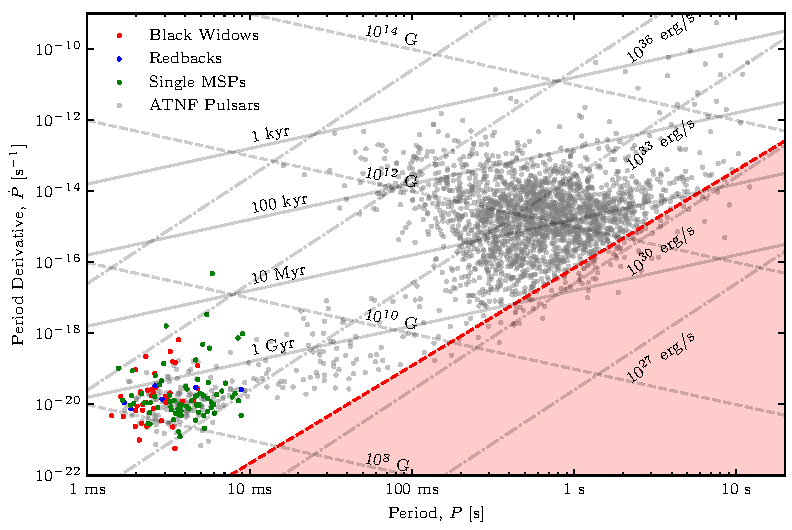
\includegraphics[width=0.8\textwidth]{figs/PPdot-diagram.pdf}
    \caption{The $P-\dot P$ diagram showing the population of pulsars. The the milisecond pulsar subclasses are colour coded. The red region represents the death line, where pulsars are theortically no longer able to emit radio waves.}
    \label{fig:p-pdot}
\end{figure}

\subsection{The Properities of Pulsars}

The following section gives a breif non-exhaustive overview of some of the key properities of pulsars. 

\subsubsection{Neutron Star Radius \& Mass}

Understanding the mass of pulsars are important for understanding their evolution and equation of state. \cite{oppenheimer_massive_1939} derived a canonical mass limit of neutron stars to be 1.4 $\smass$, but expermientally this has been shown to be higher with the largest mass of a pulsar being $\sim 2.35 \smass$ \citep{Romani_2022}. The mass-radius relationship of a pulsar is defined by an equation of state and a maximum mass limit. Redshifts and gravatational effects observed in pulsars exhbit the observed temperture and flux to be smaller than the actual value. The observed radius $R_\text{obs}$ can be described as follows \citep{pulsar_handbook}, 

\begin{equation}
    R_\text{obs} = \frac{R}{\sqrt{1 - \frac{2GM}{Rc^2}}} = \frac{1}{R} \sqrt{1 - \frac{R_s}{R}}
\end{equation}

where $R$ is the pulsar's radius and M is the gravatational mass, $G$ is the gravatational constant, $c$ is the speed of light and $R_s$ is the Schwarzschild radius. \\ 
The lower limit of the neutron star radius is decribed by 

\begin{equation}
    R_\text{min} \simeq 1.5 \ R_s = \frac{3GM}{c^2} = 6.2 \ \text{km} \left( \frac{M}{1.4 \smass} \right)
\end{equation}

Opposite to this upper limit of the radius is obtained by requiring that there is stability against breaking up due to centrifulgal forces. This gives \cref{eq:radius-max} following as described in \cite[p.~58]{pulsar_handbook}. 

\begin{equation}
    R_\text{max} \simeq \left(\frac{GMP^2}{4 \pi^2}\right)^{1/3} = 16.8 \ \text{km} \left( \frac{M}{1.4 \smass} \right)^{1/3} \left( \frac{P}{\text{ms}} \right)^{2/3}
    \label{eq:radius-max}
\end{equation}

Most pulsars are observed to have radii in the range of 10 - 15 km \citep{lattimer_neutron_2001}, giving them the unique position of 'almost' black holes. 

\subsubsection{Spin Evolution}
One of the most unique characterstics of pulsars is the spinning that they exhibit. Understanding the spin evolution gives insight into many parameters of the pulsars most notable the stage of their evolution. Pulsar's begin their life in the upper end of the $P-\dot P$ diagram and slowly move down and to the right as they age due to a loss in rotational energy, commonly referred to as spin-down luminosity. The spin-down $(\dot E)$ is decribed as follows  \citep[p.~59]{pulsar_handbook}, 

\begin{equation}
    \dot E  = - \dfrac{dE_{\text{rot}}}{dt} = 4\pi^2 I \dot P P^{-3}
    \label{eq:spin-down-energy}
\end{equation}

Where $I$ is the moment of inertia. It is important to note that the energy loss that is converted into radio emmision is almost negligable in comparison to the total energy loss from spin down. 

% \subsubsection{Radio Emission Beam}

% Pulse width

% \begin{equation}
%     \cos \rho = \cos \alpha \cos (\alpha + \beta) + \sin \alpha \sin (\alpha + \beta) \cos \left( \frac{W}{2} \right)
% \end{equation}

\subsubsection{Braking Index}

Pulsar's have strong magnetic dipoles, according to classic mechanics a rotating magnetic doplole that exhibts a moment, $|m|$ emits an electromagnetic wave at the pulsars rotation frequency \citep[p.~60]{pulsar_handbook}. The dipoles radiation power is characterized by, 

\begin{equation}
    \dot E_{\text{dipole}} = \frac{2}{3c^3} |m|^2 \omega^4 \sin^2 \alpha
\end{equation}

Where $\alpha$ is the angle between the magnetic axis and the rotation axis. Equating the above equation to the loss of rotational energy described in \cref{eq:spin-down-energy} gives the following for the expected evolution of the period, 

\begin{equation}
    \dot \Omega = - \frac{2}{3Ic^3} |m|^2 \Omega^3 \sin^2 \alpha
\end{equation}

This is more commonly written ass a power law, 

\begin{equation}
    \dot \nu = -K \nu^n 
    \label{eq:spin-down-power-law}
\end{equation}

\Cref{eq:spin-down-energy} in terms of the period is, $\dot P = K P^{2-n}$. Since this is a first order differential equation, the solution can be intergrated and given a constant, $K$ which provides and expression of age. 

\begin{equation}
    T = \frac{P}{(n-1)\dot P} \left\{ 1 - \left( \frac{P_0}{P} \right)^{n - 1} \right\} 
    \label{eq:age-full}
\end{equation}

Here $P_0$ is the initial period of the pulsar. Commomly an assumption is made that the current perios is much greater than the intial period $(P_0 \ll P)$. If it is also assumped that the pulsar is spinning down to due dipole magnetic radiaiton ($n=3$), \cref{eq:age-full} can be simplified into a charaactertic age. 

\begin{equation}
    \tau_c \cong 15.8~\text{Myr} \left( \frac{P}{s} \right) \left( \frac{\dot P}{10^{-15}} \right)^{-1}
\end{equation}

The above estimation for a pulsars age is known to be inconsistent with theorey to varying degrees. In cases where a Supernovae has been observed and produced a pulsar the age is known to a much higher degree of accuracy. The Crab pulsar is one such example with an observed Supernova event in 1054 AD by Chinese astronmers \citep{kaspi_chandra_2001}. %Supernoave remnants are also used to estimate the age of pulsars. 

\subsubsection{Dispersion Measure}

The interstellar medium (ISM) is a complex mixture of gas, dust and magnetic fields that fills the space between stars in a galaxy. Given that the ISM is a cold and ionised plasma any electromagnetic radiation will undergo a frequency-depedant index of refraction as they propagate. The following equation describes the refractive index of the ISM neglciting Galactic magnetic field \citep[p.~85]{pulsar_handbook},

\begin{equation}
    \mu = \sqrt{1 - \left( \frac{f_p}{f} \right)^2}
    \label{eq: ism-refractive-index}
\end{equation}

Where $f_p$ is the plasma frequency, $8.5 ~\text{kHz} \left(n_e/\text{cm}^{-3} \right)^{1/2}$ and $f$ is the frequency of the observed radiation. \\ If the refractive index of the ISM $\mu < 1$ then it can be assumed that the group velocity of the radiation is $v_g = c\mu$ which is sub light speed. The path of radiotion from a pulsar to the observer will be delayed in time with respect to a infinite frequecy by an amount, 

\begin{equation}
    t = \left( \int^d_0 \frac{dl}{v_g} \right) - \frac{d}{c}
\end{equation}

If is assmumed to be $f_p \ll f$, $\mu$ can be approximated.

\begin{equation}
    t = \frac{1}{c} \int^d_0 \left(1 + \frac{f_p^2}{2f^2} \right) dl - \frac{d}{c}  = \frac{e^2}{2 \pi m_e c} \dfrac{\int^d_0 n_e ~dl}{f^2} \equiv \mathcal{D} \cdot \dfrac{\text{DM}}{f^2}
\end{equation}

Where $\mathcal{D}$ is the dispersion constant and $\text{DM}$ is the dispersion measure. Each are commonly expressed as follows, $\mathcal{D}= 4.15 \times 10^3 ~\text{MHz}^2 ~\text{pc}^{-1} ~ \text{cm}^3 ~\text{s}$ and $\text{DM} = \int^d_0 n_e ~dl ~\text{cm}^{-3} ~\text{pc}$. This definition was adapted from \citet[p.~86]{pulsar_handbook} and \cite{taylor_recent_1977}.

\subsection{Pulsar Subclasses}
Following breif overview of the properities of pulsars, this section will give a breif overview of the subclasses of pulsars. The population of pulsars can be broken down into subclasses based on unique patterns in their properities. The main subclasses\footnote{This is a non-exhaustive list.} are as follows:

\begin{enumerate}
    \item Normal Pulsars: These are the most common type of pulsars. They are characterized by their regular pulses and are often observed in radio wavelengths. They are also known as radio pulsars. %they cover central region of the $P-\dot P$ diagram.

    \item Rotating Radio Transients (RRATs): These are a subclass of pulsars that were initially discovered through their sporadic radio bursts rather than regular pulses. They exhibit irregular and infrequent radio emission.

    \item Magnetars: While not exclusively pulsars, magnetars are highly-magnetized neutron stars that can also emit pulsed radiation. They are characterized by extremely strong magnetic fields, much more intense than typical pulsars.

    \item Binary Pulsars: These are pulsars that are in orbit around another star, usually a normal (non-neutron) star. The interaction with the companion star can have significant effects on the pulsar's behavior.
    
    \item Millisecond Pulsars (MSPs): These are pulsars with very short rotation periods, typically less than 10 milliseconds. They are believed to be old pulsars that have been spun up by the accretion of mass from a companion star in a binary system.

    \item X-ray Pulsars: Pulsars that emit pulsed X-ray radiation fall into this category. These pulsars are typically observed in binary systems where the pulsar accretes matter from its companion star, leading to X-ray emission.

    \item Anomalous X-ray Pulsars (AXPs) and Soft Gamma-ray Repeaters (SGRs): These are closely related to magnetars and are characterized by their intense and variable X-ray and gamma-ray emission. They are believed to be neutron stars with extremely strong magnetic fields.
\end{enumerate}

\subsection{Spider Pulsars}

The type of pulsar that is of interest to this project is a subclass of transional miliscond pulsars known as Spider Pulsars. Spider pulsars fall into two categories depending on their orbiting companion. The first category are known as Black Widow pulsars segreated based on their companion mass falling in the range of 0.01 - 0.05 $\smass$ with a compantion orbital period ($P_B$) of less than 10 hours (citation). The second category are known as Redback pulsars and have a companion mass of 0.2 $\smass$ or greater with a $P_B$ of less than 1 day (citation). \\ 

\begin{figure}
    \centering
    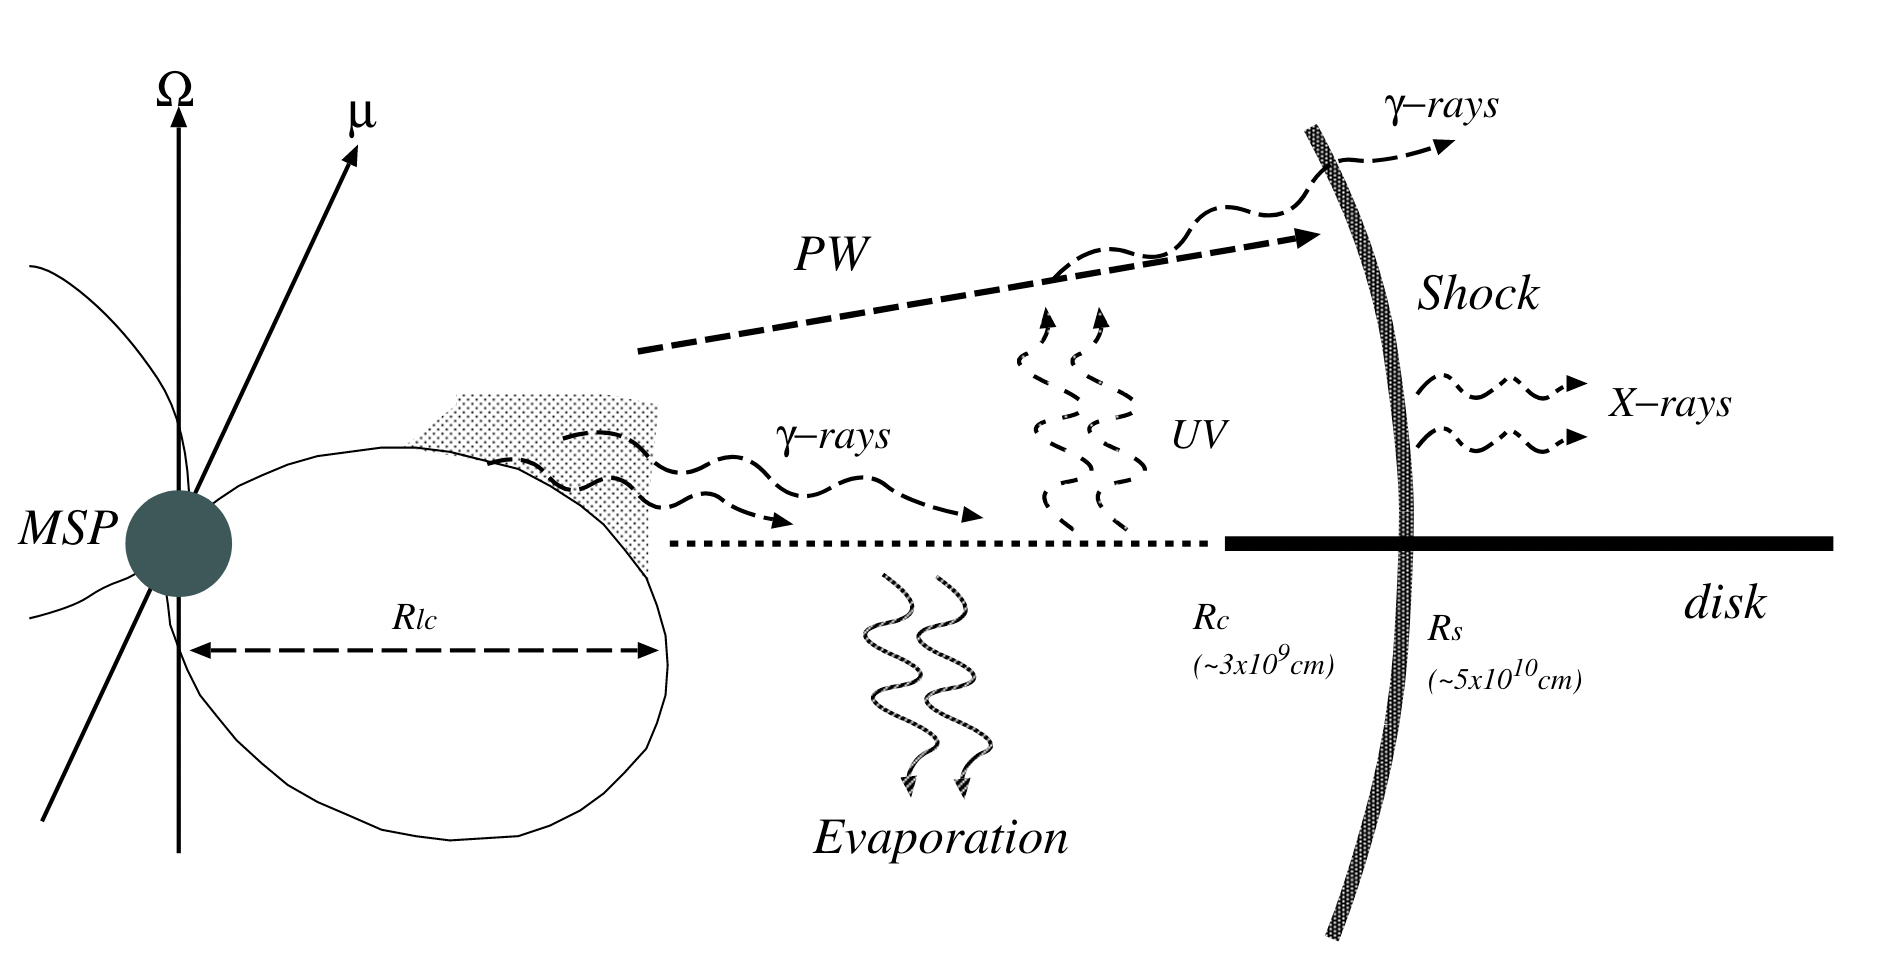
\includegraphics[width=0.8\textwidth]{figs/theory/redback-multiwavelength-emission.jpg}
    \caption{Figure taken from \cite{takata_multi-wavelength_2014}. Example of multiwavelength emission from a Redback pulsar.}
\end{figure}

It is thought that most milisecond pulsars are formed through the accretion of matter from a evolved compact binary system, the $\sim 30\%$ found in isolation are thought to have ablated their companion star to the point of dissapaction (citation). Matieral being thrown off the pulsar causes the radio emission to be eclipsed via scattering and absorption, for a segment of the companion's orbit. Rebacks systems exhibit both positive and negative period derivatives that are larger than the expected gravatiational radiation and is thought to a-rise from the interaction of the companion's magnetuc field and the pulsar's wind (citation). \\
Redback pulsars have been observed in two transional states ablation and accretion states (citation). These states are on sub year timescales. The transition in stages sees the magnitude of optical emission to increase by about $\sim 1$ order of magnitude. Studying optical emission from redback pulsars informs on the heating of the companion. Roche-lobe filling fraction and the mass of the system (citation). \\ Black widow pulsars have been observed to have little to no observable X-ray emission (citation). However, redaback's have been shown to exhibit much more x-ray emission in their thermal spectra with consistent double peaks obseravble when the pulsar is at inferior conjunction (citation). \\
The observed companions of redbacks are mostly faint stars with tempertures around X on the farside of the star from the pulsar. The companion's interaction with the pulsar dominates the thermal spectrum of spider pulsars from the present heating between the two. \\
X-ray emission from redbacks shows hard X-ray spectra that follows a power law with photon indices $(\Gamma)$ around 1 - 1.3. The energy of the thermal spectra in the X-ray is higher than what is expected from shock acceleration. Some models suggest tgat a wind-wind shock betweeb the pulsar and companion. However, this approach would require the wind momentum of the pulsar to be much weaker than the companion's. But similarly with the optical emission, the X-ray emission may be influenced by the magnetic field of the companion.  

\subsection{Why study Redback Pulsars?}

Redback pulsars have a number of interesting science cases. Redbacks undergo a range of phenomena, including radio and X-ray pulsations, accretion processes, and periodic eclipses as the companion star passes in front of the pulsar. Their study also provides valuable insights into the evolution of binary systems, the behavior of pulsars, and the physics of accretion processes.. Due to their transitional nature they provide a glimpse into the evolution of pulsars in the latter stages of their evolution. Pulsars are also used as tools to study theories of gravity, the interstellar medium and probe for gravatational waves. 

\subsection{Other exotic transients}

Redbacks themselves exotic transients, but there are many other clases of radio exotica that are of interest for the community. In this project work has also been carried out on an array of various radio transients and related objects. This includes the search for extraterrestrial intellgience (SETI), the study of M and Brown dwarf radio flares and the probing of potential radio emission from exoplanets. 

\subsubsection{Dwarf Stars}

\subsubsection{SETI}

The search for life elsewhere in the universe as always been a burning question for many astronmers throughotu history, even more the previlance of intellgient life in the universe. Since the 1960's there has been consisent surveys, mainly in radio that look for signals of artifical origin, commonly referred to as technosignature. These signatures are thought to be similar to that of radio signals produced artifically on Earth. These signals are mainly thought to be narrowband drifiting radio emission that would be produced by a transmitter leaking into space. To date there has been no positive detection of a technosignature. Similar to dark matter searches, the lack of detections has allowed for limits to be placed on the number of previlance of civilizations in the galaxy.

\begin{equation}
    N = R_* \cdot f_p \cdot n_e \cdot f_l \cdot f_i \cdot f_c \cdot L
\end{equation}


% \subsubsection{4FGL J0523-2529}

% \subsubsection{4FGL J2054-6904}

\section{Work This Far}
\subsection{Search for Extraterrestrial Intelligence}
\subsection{M-dwarf Radio Flares}
% \section{Professional Development}

% Sine the beginning of my PhD I've actively been taking steps as a to develop my skills for a career in research. This takes the form of completing classes, attending conferences and giving presentations on my work to date. \\ 

% As part of my mandated learning credits both took and audited the following modules. 

% \begin{enumerate}
%     \item Overlaps at the Frontiers of
% Astrophysics, Cosmology and Particle Physics \hfill (Winter School)
%     \item C Programming \hfill (Audited) 
%     \item Programming with CUDA \hfill (Audited) 
    
% \end{enumerate}

\section{Summary}

\bibliography{frb,pulsar}       % Multiple bib files.

\end{document}

